% Offizielle Beispieldatei für beamer-Vorlage aus tubslatex Version 0.3beta2
\documentclass[fleqn,11pt,aspectratio=43]{beamer}

\usepackage[english]{babel}
\usepackage[utf8x]{inputenc}
\usepackage{graphicx}
\usepackage{bm} 
\usepackage{amsmath}
\usepackage{xcolor}
\definecolor{DGTU}{HTML}{760054}

\usepackage{bbm} %for probability notation#


\usetheme[%
  nexus,%        Nexus Fonts benutzen
  lnum,%         Versalziffern verwenden
  %cmyk,%<rgbprint>,          Auswahl des Farbmodells
  green,%<blue/orange/green/violet> Auswahl des Sekundärfarbklangs
  medium,%<dark,light,medium>        Auswahl der Helligkeit
  colorhead,%    Farbig hinterlegte Kopfleiste
  colorfoot,%    Farbig hinterlegt Fußleiste auf Titelseite
  colorblocks,%   Blöcke Farbig hinterlegen
  %nopagenum,%    Keine Seitennumer in Fußzeile
  %nodate,%       Kein Datum in Fußleiste
  tocinheader,%   Inhaltsverzeichnis in Kopfleiste
  %tinytocinheader,% kleines Kopfleisten-Inhaltsverzeichnis
  %widetoc,%      breites Kopfleisten-Inhaltsverzeichnis
  %narrowtoc,%    schmales Kopfleisten-Inhaltsverzeichnis
  %nosubsectionsinheader,%  Keine subsections im Kopfleisten-Inhaltsverzeichnis
  %nologoinfoot,% Kein Logo im Fußbereich darstellen
  ]{tubs}

% Titelseite
\title{A Statistical Approach for the Fusion of
Data and Finite Element Analysis in
Vibroacoustics}
\subtitle{Half-time report}
\author{Lucas Hermann}
% Titelgrafik, automatisch beschnitten, Weitere Optionen: <scaled/cropx/cropy>
%\titlegraphic[cropped]{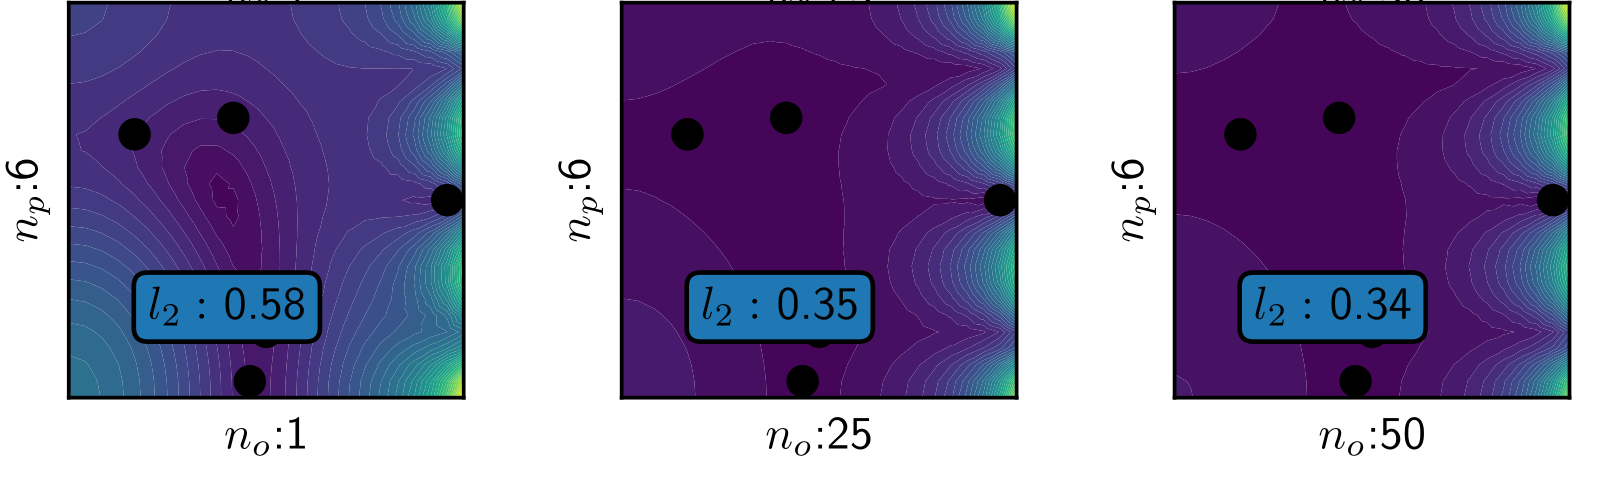
\includegraphics{titlepicture.png}}
\titlegraphic[scaled]{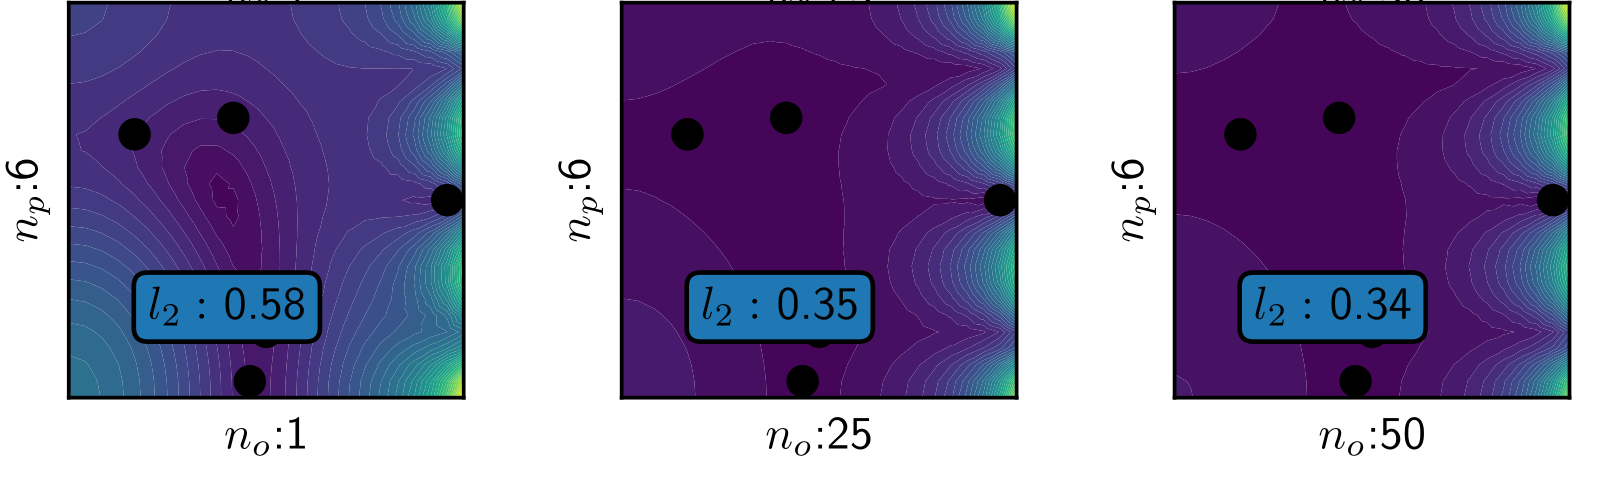
\includegraphics{titlepicture.png}}

% Logo, dass auf Titelseiten oben rechts und auf Inthaltsseiten unten rechts
% dargestellt wird. Es wird jeweils automatisch skliert
\logo{
\includegraphics{InA-Logo-rgb.pdf}}
%\logo{Institut für Unkreativität\\und Schreibschwäche}

\begin{document}

\begin{frame}[plain]
\titlepage
\end{frame}
\begin{frame}{Content}
\tableofcontents[part=1]

\tableofcontents[part=2]

\tableofcontents[part=3]
\end{frame}
\part{Objectives}

\begin{frame}[plain]
  \partpage
\end{frame}


\section{Objectives}



\begin{frame}{Objectives}

statFEM:
\begin{itemize}
  \item Merge FEM and data while quantifying uncertainty:
   Apply statFEM to an FEM solution to reduce the model error
      
 
 % \begin{itemize}
  %  \item Unterpunkte ebenfalls
   % \item Allerdings etwas kleiner
  %\end{itemize}
\end{itemize}

\begin{figure}[h]
\begin{center}
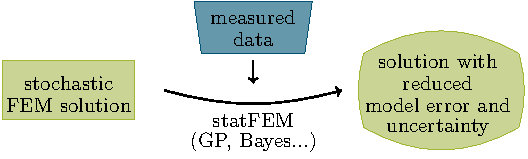
\includegraphics[scale=1]{intro}
\end{center}
\end{figure}

\end{frame}


\begin{frame}{Objectives}
The goal of the thesis is:
\begin{itemize}
	\item to understand statFEM
 	\item to apply statFEM to vibroacoustics using the Helmholtz equation
  \item to provide a means to use sparse sensor data to improve the accuracy of an FEM solution
  \item to use a non-parametric approach to increase the accuracy of the solution without touching the FEM itself
\end{itemize}

\end{frame}

\part{Prerequisites}
\begin{frame}[plain]
  \partpage
\end{frame}





\section{Prerequisites}




\subsection{Modeling data}
\begin{frame}{Prerequisites: Data}

\begin{block}{Statistical Model}
The vector of measured data $\bm{y}$ can be described as a combination of different parts:
\begin{equation}
\bm{y} = \textcolor{DGTU}{\bm{z}} + \textcolor{olive}{\bm{e}} = \textcolor{DGTU}{\rho \bm{P} \bm{u} + \bm{d}} + \textcolor{olive}{\bm{e}}
\end{equation}
\end{block}
$\textcolor{DGTU}{\bm{z}}$: The true solution\\
$\textcolor{olive}{\bm{e}}$: Measurement error\\
$\rho \bm{P} \bm{u}$: Scaled projected FEM solution\\

$\bm{d} \sim \mathcal{GP}(\bar{\bm{d}}, C_d)$: Model mismatch error
\end{frame}


\subsection{Gaussian Processes}
\begin{frame}{Prerequisites: Gaussian Processes}
\begin{block}{Gaussian Processes:}
A GP $\bm{u} \sim \mathcal{GP}(\bar{\bm{u}},C_u)$ is a distribution of functions. It is defined by a mean $\bar{\bm{u}}$ and a covariance matrix $C_u$. It is basically just a multivariate Gaussian distribution.

\end{block}
\begin{figure}[h]
\begin{center}
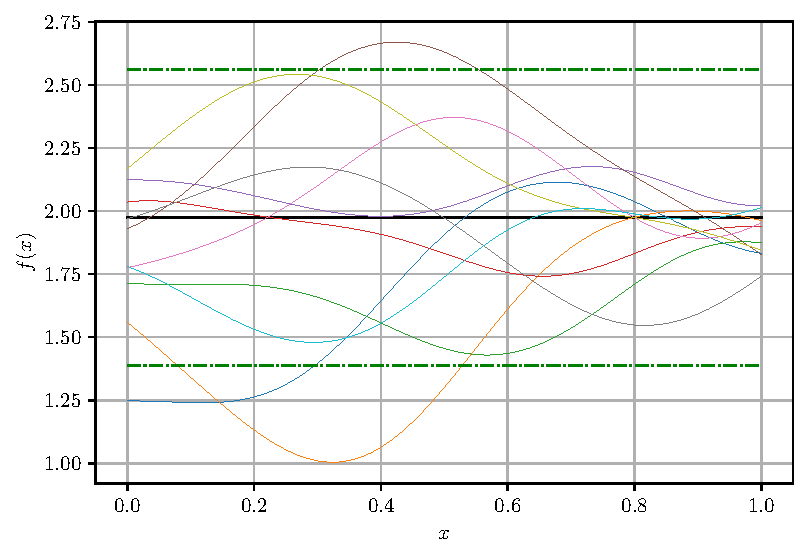
\includegraphics[width=0.6\textwidth]{sqexp_f_sampled}
\end{center}
\end{figure}

\end{frame}

\begin{frame}{Prerequisites: Gaussian Processes}
\begin{block}{Squared Exponential Kernel:}
A kernel is a \emph{covariance function}.  It continuously describes the covariance between different points in the calculation domain and describes the expected behaviour of the approximated function.
\begin{equation}
k_{SE} = \sigma \exp \left( -\frac{||x-x'||^2}{2l^2} \right)
\end{equation}
\end{block}
$\sigma$: standard deviation\\
$l$: distance measure\\
Evaluating the kernel at a defined set of points (e.g. nodes in an FEM mesh) yields the covariance matrix.
\end{frame}

\subsection{Bayesian Inference}
\begin{frame}{Prerequisites: Bayesian Inference}
\begin{block}{Bayes' law:}
Conditioning a distribution $\bm{u}$ on data $\bm{y}$ requires a prior for the distribution $p(\bm{u})$ and a likelihood for the data $p(\bm{y}|\bm{u})$.
\begin{equation}
p(\bm{u}|\bm{y}) = \frac{p(\bm{y}|\bm{u})p(\bm{u})}{p(\bm{y})}
\end{equation}
\end{block}
The prior is the stochastic FEM solution.\\
The likelihood can be derived from the statistical model ($\bm{y} = \textcolor{DGTU}{\rho \bm{P} \bm{u} + \bm{d}} + \textcolor{olive}{\bm{e}}$) in which all components are Gaussian.\\
The marginal likelihood $p(\bm{y})$ is the probability for the data averaged over all possible prior solutions.
\end{frame}



\begin{frame}{Prerequisites: Bayesian Inference}
Assuming the stochastic FEM solution to be a GP, the posterior GP can be infered using the statistical model for the data.
\begin{block}{Inference of the posterior GP:}
The posterior solution is going to be a GP: \\
$\bm{u}_{|y} \sim \mathcal{GP}(\bar{\bm{u}}_{|y}, C_{u|y})$.
\begin{equation}
\bm{\bar{u}}_{|y} = C_{\bm{u}|\bm{y}} \left(   \rho P^T  (C_d + C_e)^{-1}  y  +  C_u^{-1}  \bar{u}   \right)
\end{equation}
\begin{equation}
C_{\bm{u}|\bm{y}} = \left(      \rho^2  P^T   (C_d + C_e)^{-1}  P  +  C_u^{-1}    \right)^{-1} 
\end{equation}
\end{block}
Using an optimization method, the hyperparameters for $C_d$ are determined.

\end{frame}


\part{The statFEM procedure}
\begin{frame}[plain]
  \partpage
\end{frame}


\section{1D example}
\subsection{Setting}

\begin{frame}{Setting: 1D Poisson}
To test the methods and code, the well-known Poisson example was solved in 1D.
\begin{block}{Weak form:}
The uncertainty is in the source term: $f \sim \mathcal{GP}(\bar{f}, C_f)$
\begin{equation}
-\int_{\Omega} \nabla p \cdot \nabla v \,\mathrm{d}x = \int_{\Omega} fv \,\mathrm{d}x
\end{equation}
\end{block}
      	\begin{figure}[h]
		\begin{center}
		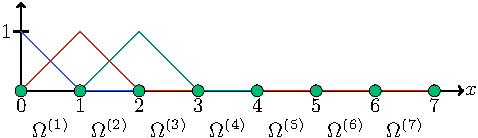
\includegraphics[width=0.6\textwidth]{1dDomain}
		\end{center}
		\end{figure}

\end{frame}


\subsection{FEM solution}
\begin{frame}{FEM solution: 1D Poisson}
The FEM solution serves as a prior and is modeled as a GP with a mean and variance. Arbitrarily many samples can be drawn from it.
      	\begin{figure}[h]
		\begin{center}
		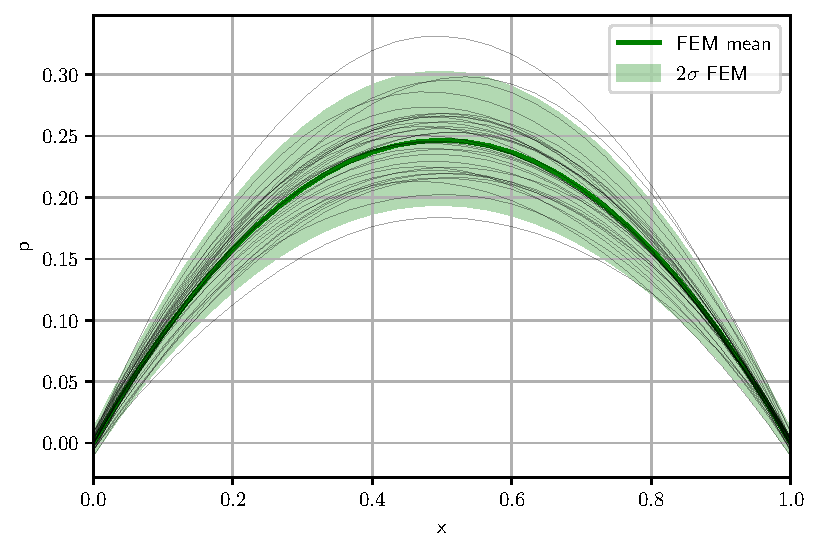
\includegraphics[width=0.7\textwidth]{1DFEMprior}
		\end{center}
		\end{figure}

\end{frame}


\subsection{Inference}
\begin{frame}{Infered solution: 1D Poisson}
1 sensor, 1 observation
      	\begin{figure}[h]
		\begin{center}
		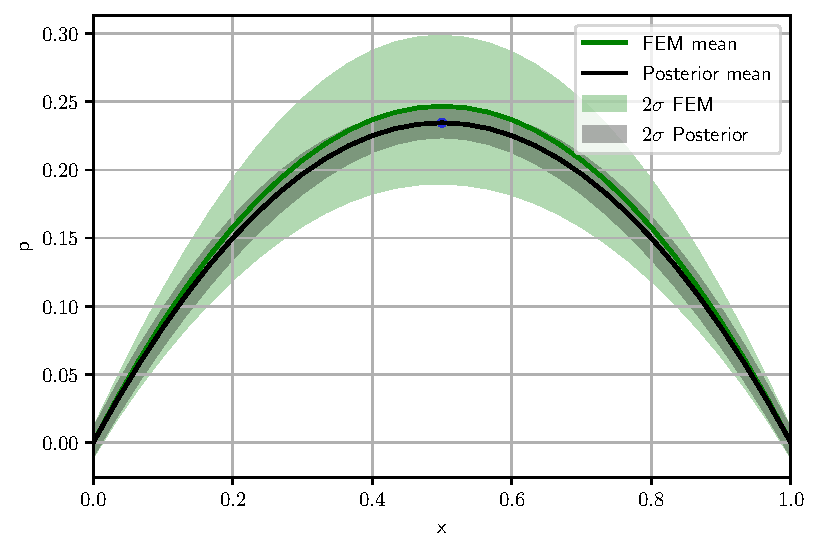
\includegraphics[width=0.7\textwidth]{1DPost_1P1O}
		\end{center}
		\end{figure}

	\end{frame}


\begin{frame}{Infered solution: 1D Poisson}
4 sensors, 1 observation each
      	\begin{figure}[h]
		\begin{center}
		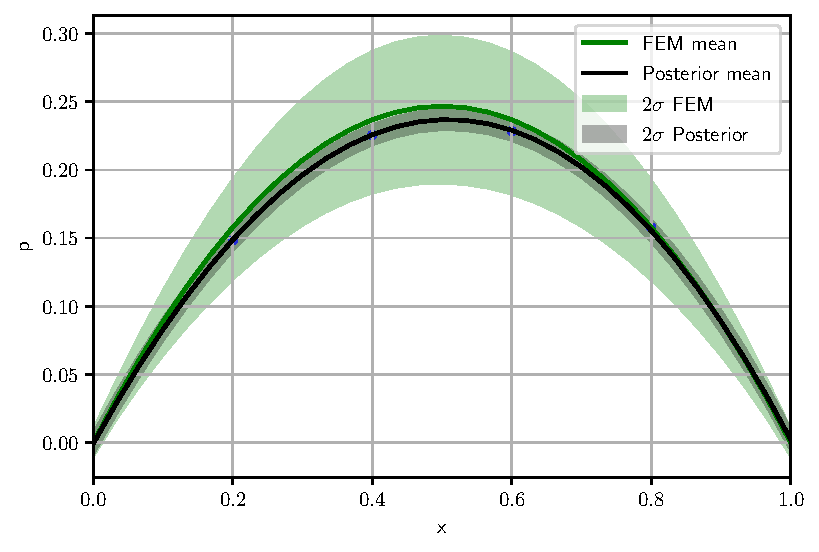
\includegraphics[width=0.7\textwidth]{1DPost_4P1O}
		\end{center}
		\end{figure}

	\end{frame}

\begin{frame}{Infered solution: 1D Poisson}
4 sensors, 20 observations each
      	\begin{figure}[h]
		\begin{center}
		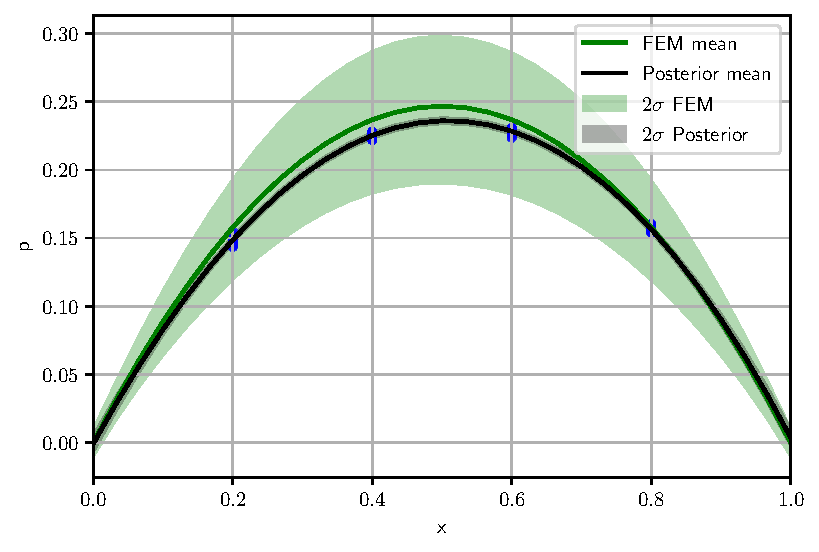
\includegraphics[width=0.7\textwidth]{1DPost_4P20O}
		\end{center}
		\end{figure}

	\end{frame}

\begin{frame}{Infered solution: 1D Poisson}
Only partial data available: FEM prior still determines overall shape
      	\begin{figure}[h]
		\begin{center}
		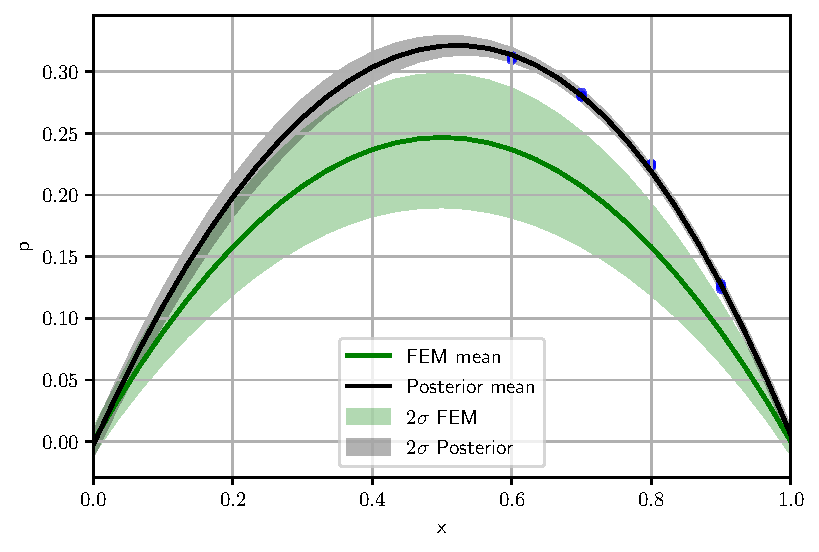
\includegraphics[width=0.7\textwidth]{1DPost_RightSide}
		\end{center}
		\end{figure}

	\end{frame}
\section{2D Helmholtz}
\subsection{Setting}

\begin{frame}{Setting: 2D Helmholtz}
\begin{block}{Weak form:}
The \textcolor{DGTU}{uncertainty} is in the boundary term.
\begin{equation}
-\int_{\Omega} \nabla p \cdot \nabla v \,\mathrm{d}\Omega + \textcolor{DGTU}{\oint_{\Gamma} v \nabla p  \,\mathrm{d}\Gamma}+ \int_{\Omega} k^2 pv \,\mathrm{d}\Omega = 0
\label{eqn:WeakHelmholtz}
\end{equation}
\end{block}

\begin{columns}[onlytextwidth]
    \column{0.5\textwidth}
    \begin{block}{Neumann boundary:}
      $\oint_{\Gamma_N} v (\rho \omega^2 \textcolor{DGTU}{\vec{D}}\vec{n})  \,\mathrm{d}\Gamma$\\
      $\textcolor{DGTU}{\vec{D}}$: Piston displacement
          \end{block}
          1D boundary function $\textcolor{DGTU}{D(y)}$: $\textcolor{DGTU}{D \sim \mathcal{GP}(\bar{g}, C_g)}$
  %    For $\vec{U} = 0$: Natural (reflecting) BC on $\Gamma_{N0}$
    \column{0.5\textwidth}
      	\begin{figure}[h]
		\begin{center}
		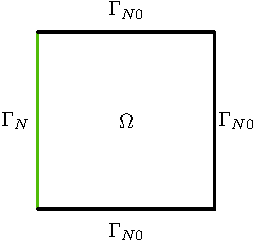
\includegraphics[width=0.8\textwidth]{BCsThesis1}
		\end{center}
		\end{figure}
  \end{columns}
\end{frame}


\subsection{FEM solution}
\begin{frame}{FEM solution: 2D Helmholtz}
The FEM solution serves as a prior and is modeled as a GP with a mean and variance. Arbitrarily many samples can be drawn from it. 
      	\begin{figure}[h]
		\begin{center}
		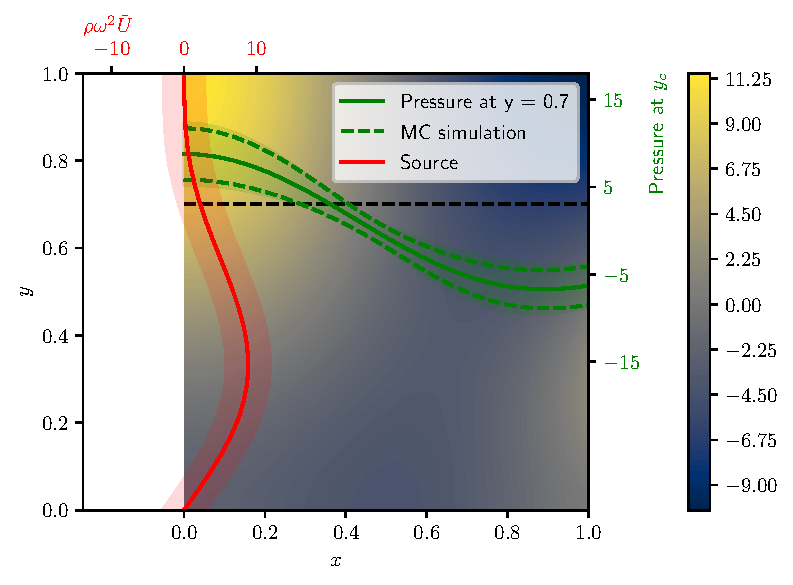
\includegraphics[width=0.7\textwidth]{2DFEMprior}
		\end{center}
		\end{figure}

\end{frame}

\subsection{Inference}
\begin{frame}{Inferred solution: 2D Helmholtz, Variance fields}
Variance drops with increasing number of sensors and/or number of observations
      	\begin{figure}[h]
		\begin{center}
		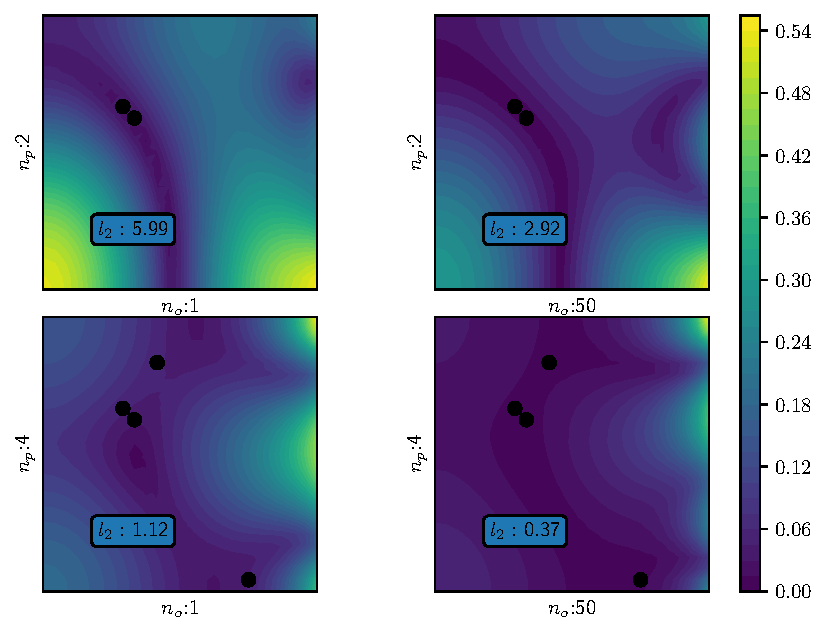
\includegraphics[width=0.7\textwidth]{VarField_Posterior}
		\end{center}
		\end{figure}

	\end{frame}


\begin{frame}{Inferred solution: 2D Helmholtz}
1 sensor, 1 observation. Data "observed" on a 75\% scaling of the FEM prior.
      	\begin{figure}[h]
		\begin{center}
		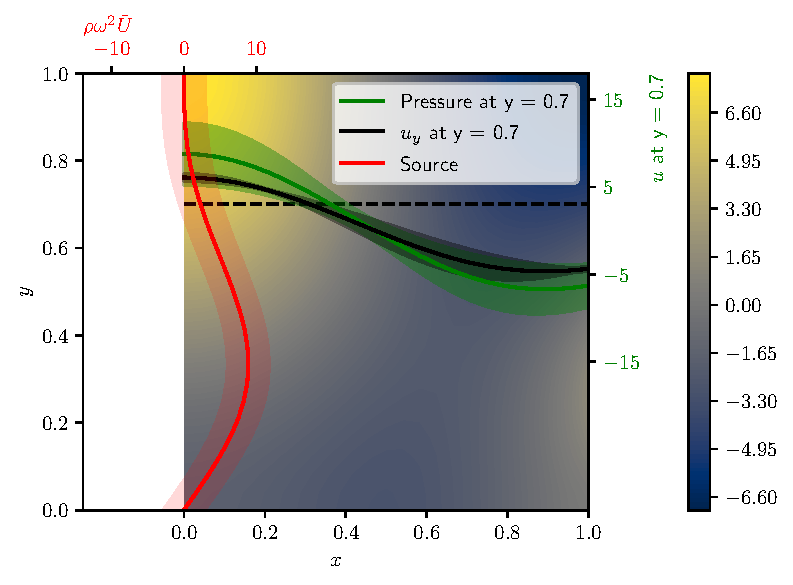
\includegraphics[width=0.7\textwidth]{SolutionCustomPosterior1P1O}
		\end{center}
		\end{figure}

	\end{frame}

\begin{frame}{Inferred solution: 2D Helmholtz}
4 sensors, 50 observations. Data "observed" on a 75\% scaling of the FEM prior.
      	\begin{figure}[h]
		\begin{center}
		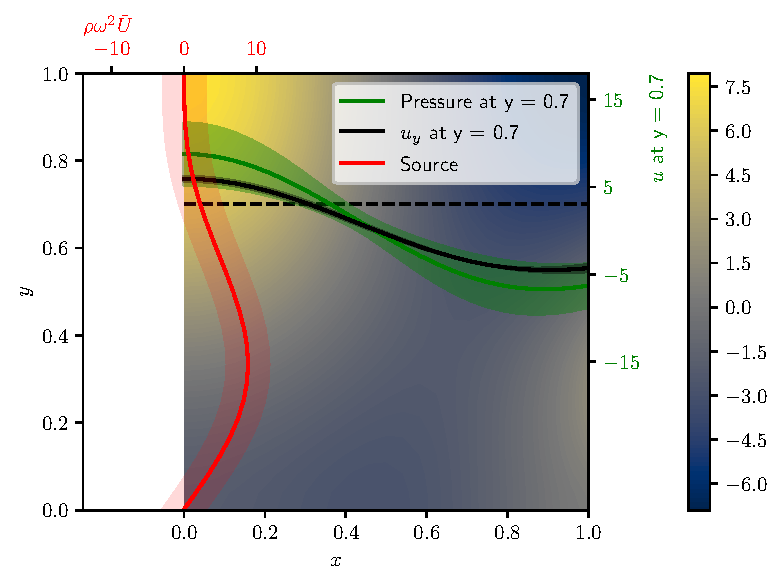
\includegraphics[width=0.7\textwidth]{SolutionCustomPosterior4P50O}
		\end{center}
		\end{figure}

	\end{frame}


\section{Outlook}

\part{Outlook}
\begin{frame}[plain]
  \partpage
\end{frame}

\begin{frame}{Status}

\begin{itemize}
\item I understood the basics and began documenting
\item A 1D proof of concept works well
\item The code for the Helmholtz solver works but needs some iterations:
	\begin{itemize}
	\item plausibility checks
	\item numerical experiments
	\item explore and find limits of the method
	\end{itemize}
\item documentation is at $\sim$ 50\%
\item further work could be done, if there is time
\end{itemize}

	\end{frame}



\begin{frame}{Timeline}

      	\begin{figure}[h]
		\begin{center}
		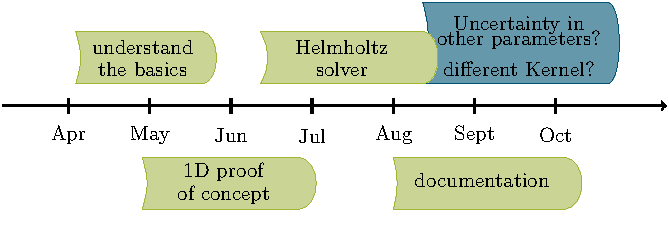
\includegraphics[width=1\textwidth]{timeline}
		\end{center}
		\end{figure}

	\end{frame}




\end{document}
